
%%%%%%%%%%%class file
\documentclass{imammb}


%this command gives the journal no. 
%
\jno{dqnxxx}
%%%%%%%%%%%%%%


%%%%%%%%%%%%%%%%%
%call  packages
\usepackage{natbib}
%%%%%%%%%%%%%%

%%%%%%%%%%%%%%%%%%

\usepackage{graphicx}
\usepackage{amsmath,amsthm,bm,mathrsfs}

%%%%%%%%%%%%%%%%%


%%%%%%%%%%%
%this files contains Theorem styles based in IMA JOURNALS
%
\input standard.tex

%%%%%%%%%%%%%


\renewcommand{\theequation}{\thesection.\arabic{equation}}
\numberwithin{equation}{section}
\def\citeasnoun{\cite}
\newcommand{\comment}[1]{}


\begin{document}

%%%%%%%%%%%%%%%%%
\title{Analyzing the propensity for superspreading using finite mixture branching process epidemic models}
\author{ {\sc Suzanne M. O’Regan and John M. Drake}\\[2pt]
Odum School of Ecology, University of Georgia, Athens GA 30602\\[6pt]
{\rm [Received on XX]}\vspace*{6pt}}
\pagestyle{headings}
\markboth{S. M. O'REGAN \& J. M. DRAKE}{\rm SUPERSPREADING USING FINITE MIXTURE BRANCHING PROCESSES}
\maketitle




%\usepackage{xcolor}
%\renewcommand{\arraystretch}{1.5}
%\usepackage{lscape}
%\usepackage{geometry}
%\usepackage{natbib}
%\usepackage{cite}
%\geometry{margin=1in}



\section{Introduction}
Heterogeneity in disease transmission arises frequently in epidemics. Individuals can vary in their ability to transmit infectious agents through biological, behavioral and environmental factors \citep{Lloyd-Smith2005-ma,Funk2010-zj, Althouse2020-dn}. Superspreading events, where one infected individual gives rise to a large number of secondary infections in a single generation, may be the source of most of the secondary cases in a population \citep{Althouse2020-dn}. Contact patterns and social structure may interact with differences in individual infectiousness, giving rise to superspreading events. For example, the first wave of the SARS CoV-2 pandemic was characterized by multiple superspreading events (e.g., \citep{Hamner2020-zt, Adam2020-xk, Lemieux2021-ow, Illingworth2021-rz}). Understanding the role of superspreading individuals in fuelling transmission in an outbreak is important for epidemic containment. 

%should this be split into multiple paragraphs? e.g contact and behavior examples, biology, environment examples. environment may need to be expanded upon further.
% Opportunities for superspreading may arise from heterogeneous contact patterns.
Individual variation in behavior, biology and environment can all induce superspreading transmission patterns. For example, \citet{Sneppen2021-mr} characterized contact heterogeneity in SARS CoV-2 transmission by distinguishing between transmission occurring in social networks consisting of mostly regular contacts (e.g., individuals encountered on a daily basis such as those within one’s household) and transmission occurring in large contact networks consisting of individuals encountered infrequently (e.g., encounters in retail stores, bars or public transport). Their modeling showed that individuals whose social network consists of high numbers of infrequently encountered individuals (e.g., retail workers) have a greater diversity of contacts and therefore greater propensity for superspreading than individuals with narrow social networks and few random contacts (e.g., remote workers). Biological factors that increase the probability of successful transmission and the contact rate per infectious individual can also induce superspreading. These include heterogeneities in shedding rate and/or viral load \citep{Goyal2021-xr}, differences in transmission mode (e.g., aerosol vs. droplet transmission \citep{Chen2021-wo}) and symptomatology (asymptomaticity/mild symptoms vs. severe symptoms \citep{ Illingworth2021-rz}). For example, if transmission occurs primarily via aerosols, more people can become infected as aerosols travel further and hang for longer in the air, in contrast with droplets that quickly fall to a surface. Frequenting crowded poorly ventilated environments where it is difficult to implement social distancing can also contribute to superspreading transmission, particularly if combined with biological factors (e.g., frequent coughing) or behavioral factors (e.g., refusal to wear a mask in crowded settings). In particular, there is a need to distinguish between heterogeneities in transmission that arise due to supershedding, which is due to biological factors, and superspreading, which arises primarily due to contact patterns \citep{Rock2014-nc}. Much of these heterogeneities are likely to impact the contact process that results in transmission.

%In sum, the probability distribution of the number of secondary infections $N$ depends on just two microlevel processes: a contact process $\{K(x)\}$ leading to infections that each infectious individual independently follows and the infectious period cumulative distribution $F_I(x)$. We note that different specifications of these processes and mixtures can induce the same GW process with mean $R_0$ and offspring distribution of N at the macro-level (Yan 2008).



%%move this paragraph elsewhere?
%In theory for branching processes of epidemics, the probability distribution of the number of secondary infections per individual depends on just two microlevel processes: a contact process leading to infections that each infectious individual independently follows and the infectious period cumulative distribution function (Yan 2008). Firstly, the process describing the cumulative number of contacts leading to infection made by an infectious individual with susceptible individuals per unit time is specified (e.g., Mode and Sleeman 2000, Yan 2008). A Poisson contact process with intensity $\lambda q$ is typically assumed, where $\lambda$ is the expected number of contacts per unit time and $q$ is the probability of infection given contact. A Poisson process implies that the time between transmission contacts (exposures leading to infection) is exponentially distributed (Mode and Sleeman 2000, Yan 2008, Diekmann Heesterbeek and Britton 2013) and thus contacts with susceptibles are effectively random. Second, a model for the infectious period is specified. For example, in Crump-Mode-Jagers (CMJ) branching processes, the infectious period for each individual is a continuous random variable. Common assumptions for the infectious period distribution include the exponential distribution, and the gamma distribution. An exponentially distributed infectious period implies that the majority of cases recover rapidly from infection. In contrast, a gamma distribution can be parameterized to have a central tendency, which more realistically describes the distribution of the infectious period for many diseases (Keeling and Rohani 2008). Mixing the Poisson contact process with the distribution of the infectious period yields a mixture distribution that describes the number of offspring (cases) per generation (Mode and Sleeman 2000, Yan 2008, Diekmann Heesterbeek and Britton 2013). Conveniently, CMJ processes have an embedded discrete-time Galton-Watson (GW) process that tracks the number of offspring per generation and governs outbreak threshold behavior \citep{Mode2000-hp}. Typically researchers simulate the number of secondary infections per individual in discrete time using an offspring distribution arising from a GW process (e.g., \citep{Lloyd-Smith2005-ma, Kucharski2015-lh, Endo2020-td, Hellewell2020-go}). Additionally, the theory of GW processes offers many analytical and computational advantages. The total number of cases arising from a single infected individual (i.e., a transmission chain) can be simulated easily, the probability of a large outbreak can be calculated and the distribution of transmission chains that go extinct can often be obtained (e.g., \citep{Blumberg2013-xv}).

%Long-tailed secondary infection distributions induce greater variability in outbreak size, which can be characterized by larger probability of observing no secondary infections, smaller probability of major epidemics, larger coefficient of variation in the number of secondary infections and greater probabilities of observing a chain smaller than a given size than for Poisson epidemics \citep{Althouse2020-dn}.

%The negative binomial distribution is the most commonly used offspring distribution for modeling superspreading events. Typically the micro-level assumptions of its underlying CMJ process are a Poisson contact process and a gamma-distributed infectious period, with the resulting mixture distribution being negative binomial e.g., \citep{Lloyd-Smith2005-ma}.

%Different microscale processes can yield the same macroscale process describiing outbreaks (e.g. Gaske, Yan, 
%maybe say could be due to heterogeneity in infection duration, or average reproductive number
 
A simple and commonly used model for superspreading events is the negative binomial distribution for the number of secondary infections per infectious individual. The negative binomial distribution can be described using a mean $R_0$ and dispersion parameter $k$. If $k$ is small, the distribution is long-tailed and its variance is greater than the mean, a property that cannot be captured using classical Poisson distributions. Long-tailed secondary infection distributions induce greater variability in outbreak sizes, larger probability of observing no secondary infections, smaller probability of major epidemics and greater probabilities of observing a chain smaller than a given size than Poisson epidemics \citep{Althouse2020-dn}. Using a negative binomial branching process allows 
the total number of cases arising from a single infected individual (i.e., a transmission chain) to be simulated easily, and analytical results from branching process theory yield the probability of a large outbreak \citep{Mode2000-hp} and the distribution of transmission chains that go extinct (e.g., \citep{Blumberg2013-xv}).  However, heterogeneous transmission is often characterized by the host population being partitioned into two or more groups, e.g., by social, biological, behavioral or environmental risk structure (Keeling and Rohani 2008, Rock et al. 2014).   Each group has distinct characteristics that affect the distribution of the total number of secondary infections per infected individual belonging to that group. For example, an important aspect of population heterogeneity that is not accounted for in the standard negative binomial model is the partitioning of the population by average contact rate. Heterogeneity can arise if a certain proportion of the population have high random mixing levels or engage in risky behavior, or if a certain proportion of the population have high shedding rates with consequent high probability of infecting others. Models for the distribution of secondary infections that combine population risk structure with realistic distributions of infection duration are currently lacking.
 
Here we study the effect of the simplest heterogeneous population structure by dividing the population into two groups that are characterized by different average total number of contacts leading to infection per unit time, i.e., two Poisson processes with different intensities. Dividing the population into subpopulations with different transmission rates gives rise to a contact process described by a finite mixture of two Poisson distributions. A finite mixture of negative binomial distributions with the same dispersion parameter arises from mixing the Poisson finite mixture with a gamma distribution for the infectious period. Then a finite mixture of geometric distributions and a finite mixture of Poisson distributions arise as special cases.  To study the effect of population structure on the stochastic characteristics of transmission at the beginning of an outbreak, we calculate the mean and variance of the secondary infection distributions, use the generating functions to calculate the probability of a major epidemic when $R_0>1$, and we derive the transmission chain size distributions conditioned on extinction. To understand how these key statistics differ from those generated assuming no contact heterogeneity, we compare the statistics obtained from the mixture distributions with those generated by a negative binomial distribution with the same mean and dispersion parameter.  To examine implications of population structure on containment, we study the effect of decreasing $R_0$ in three ways. First we alter the heterogeneous structure of the population by examining the effect of varying the transmission heterogeneity ratio $p$. We reduce the proportion of individuals with high transmission rate, which is equivalent to decreasing the proportion $p$ of the population that do not comply with stay-at-home orders or with face covering mandates, do not self-isolate when sick or decreasing the proportion of the population with high probability of transmission through viral load or shedding rate. Next we decrease the average number of additional successful contacts per generation in the superspreading cohort while keeping it fixed in the remainder, which may be viewed as decreasing their intensity of interactions (e.g., by changing the working environment). Third, we decrease baseline transmission rate in both groups simultaneously e.g., both groups wear face coverings. Our work shows that the mechanistic addition of population structure induces qualitatively different outbreak patterns from a standard negative binomial superspreading model with mean $R_0$ and dispersion parameter $k$. We show that the critical threshold for containment is different depending on whether superspreaders only are targeted or both cohorts are targeted, and which of these strategies is the most effective is context-dependent. 

%We study three finite mixtures: a model with transmission heterogeneity only (a finite mixture of two Poisson distributions) and two models with heterogeneities in transmission patterns and infection duration (finite mixtures of two negative binomial distributions and two geometric distributions).

%do they have the same variance? I think not, because p varies. The bit that is different is G''(N)
 


 %alter risk structure
 
%In summary, our key questions are:
%\begin{itemize}
%    \item Does the mechanistic addition of population structure induce qualitatively different outbreak patterns from a standard negative binomial superspreading model with mean $R_0$ and dispersion parameter $k$ assuming $R_0>1$? 
%\item How does decreasing the level of superspreading by a) changing the population structure e.g., by shifting the contact structure away from opportunistic encounters/aerosol transmission and towards regular contacts/direct contact transmission, and b) decreasing the average number of successful contacts in the superspreading cohort affect heterogeneity in outbreak patterns, and what are the implications for containment?
%\end{itemize}



\section{Methods}
%high level summary of approach
%need to introduce the base model for superspreading

\subsection{Review of standard superspreading model}

%need pmf, pgf, prob of extinction, mean and variance. 
%chain distribution formula?

%also standard superspreading model can be derived by assuming a Poisson contact process, gamma distributed infectious period and their mixture is negative binomial. 
%I don't want to be heavily critical of the model either. just want to examine how exactly superspreading arises, and deriving a more mechanistic model. 
%which arises from mixing gamma distributed infectious period with constant contact rate per infectious individual.
We begin by reviewing the derivation of the standard superspreading model in \citet{Lloyd-Smith2005-ma} and its underlying micro-level processes. 
Firstly, each individual has an expected reproductive number, defined as the average number of secondary infections per person over the course of their infectious period, and it is a random variable $\nu$. To model variation in infectiousness, individual expected reproductive numbers are gamma-distributed with mean $R_0$ and dispersion $k$. Secondly, because of demographic stochasticity in disease transmission, the reproductive number that is observed per infectious individual is a Poisson distributed random variable with mean $\nu$. Integrating over all possible individual reproductive numbers yields a negative binomial model with mean $R_0$ and dispersion parameter $k$. Alternatively, the standard negative binomial model for superspreading can be derived by assuming each infected individual follows a Poisson contact process with mean $\beta$, and each individual has a gamma-distributed infectious period with mean $1/\gamma$ and coefficient of variation $1/\sqrt{k}$. Then the mixture of these distributions is negative binomial with mean $R_0 = \beta/\gamma$ and dispersion parameter $k$ (e.g., \citep{Mode2000-hp,Diekmann2013-zu, Yan2008-jc}). If $k$ is close to zero, then the infectious period distribution is right-skewed and therefore most individuals generate 0 or 1 secondary infections since most individuals have a short infectious period. However, because the infectious period distribution has a long right-hand-tail, some individuals remain infected for long times and therefore infect many individuals over the course of their infectious period, giving rise to superspreading events. In Table \ref{tab:standardstats} we list the probability mass function, probability generating function and the statistics obtained from the negative binomial model that we use in this paper. 

We note that different micro-scale continuous processes can induce the same discrete time process at the macro-level that describes the distribution of outbreaks \citep{Mode2000-hp, Garske2008-ax, Yan2008-jc}. For example, another alternative model to the formulations specified above would be to assume that the transmission rate is a gamma distributed random variable, and the duration of infectiousness is constant, and mixing this with demographic stochasticity in contact, we again obtain a negative binomial offspring distribution with mean $R_0$ and dispersion $k$. In all of these formulations of the standard model, heterogeneity in secondary infections is caused by overdispersion in infectiousness. The model does not capture heterogeneity in population structure that could additionally induce superspreading such as the processes that divide the population into distinct risk groups (e.g., those listed in Table \ref{tab:micro}). For example, in closed settings such as professional sports teams, prisons  and care homes, the risk structure of the population may be known \textit{a priori}, e.g., the population can be divided into those who are vaccinated and unvaccinated. Here we aim to examine the micro-level processes that induce superspreading transmission, and to use them to derive a more mechanistic model. 

%We want to be more specific in how we specify risk structure

%We note that different micro-scale CMJ processes can induce the same GW process at the macro-level (Yan 2008). %Different mixtures of contact processes with the distribution of the infectious period can yield the same probability distribution for the number of secondary infections and same $R_0$.

 



%check my derivation of the chain size distribution
\begin{table}[h!] %T2
\tblcaptionnotes{Probability mass function, probability generating function and statistics for the standard negative binomial model with mean $R_0$ and dispersion parameter $k$}
{\mbox{\tabcolsep=10pt\begin{tabular}{@{}cc@{}}
\tblhead{Name & Expression \\[-11pt]}\\[-9.5pt]
Probability mass function &  $P(N=j) =  \frac{\Gamma(j+k)}{j! \Gamma (k)}  \left(\frac{k}{k+R_0} \right)^{k}\left (\frac{R_0}{k+R_0} \right )^j  $\\[3pt]
Probability generating function 
& $F(s) = (1 + \frac{R_0}{k}(1-s))^{-k}$ \\[3pt]
Variance of offspring distribution  &$V(N) = R_0(1+\frac{R_0}{k})$  \\[3pt]
Probability of extinction $s^*$ &  Solve $s=F(s)$ for $s^*$
\\[3pt]
Probability of a chain of size $y$   &$ P(Y=y) = \frac{\Gamma (k j + j -1) }{\Gamma(kj) \Gamma (j+1)}\frac{(\frac{R_0}{k})^{j-1}}{(1+\frac{R_0}{k})^{kj+j-1}}   $  \\[-9pt] \lastline
\end{tabular}
\label{tab:standardstats}
}}{}\vspace*{-2pt}%leave footnote space blank, e.g. $^a$ Iteration counts obtained with the ideal preconditioner are
%listed in columns 2--3 of Table 2\\$^b$ The negative eigenvalues
%of the preconditioned saddle point system.
\end{table}

%criticism: too coarse?
%moreover the standard model assumes that the superspreading comes from the gamma distributed infectious period only and the mixing with poisson is due to the coarse assumption of demographic stochasticity (in what?) or it comes from individual reproduction numbers that are gamma distributed. and what is an individual reproduction number? individual contact rate * individual inf period. The inf period being drawn from gamma....but they assume everyone in the population has the same contact rate (i.e. it is not an rv) 
%neg binom macroscale (generation) Here we look at microscale processes at the individual level 

%gamma distribution with small k: most people recover quickly, but a few take extremely long time to recover. 

%mechanistic derivation? the standard model for superspreading is the negative binomial with mean R0 and dispersion k. There are a couple of things I can see. For example Lloyd Smith et al used a neg binom model for superspreading by arguing that individual reproductive numbers were gamma distributed with mean R0 and dispersion parameter k and demographic stochasticity was Poisson distributed. The resulting Poisson-gamma mixture distribution is a negative binomial. On the other hand, a negative binomial can be derived by gamma distributed infectious period with mean 1/gamma and CV 1/k and Poisson contact process with intesnity beta. That model would have the superspreading component captured by the dispersion parameter - disadvangtage since it suggests 

%see Nishiura
%want to also argue our model gives rise to a gW branching process that wesimulate

\subsection{Mechanistic superspreading model}

%different microlevel processes can lead to superspreading at the macrolevel. %To model superspreading, we need to consider what happens on the microlevel

 %[High level overview of modeling approach]
 
 %should i define microlevel processes before this paragraph? 
We distinguish between superspreading and regular transmission.  Infectious individuals may have superspreading transmission characteristics or they may have non-superspreading (i.e., regular) transmission characteristics. Table \ref{tab:micro} summarizes examples of micro-level processes that may underpin heterogeneous transmission in a population. Sources of heterogeneity can either partition the population into distinct risk groups (e.g., by occupation) or they can be continuous (e.g., by duration of infectious period) and may either affect the contact process or the duration of infectiousness. Here we develop a branching process model that combines both binary and continuous sources of heterogeneity. Specifically, we develop a model of a Crump-Mode-Jagers (CMJ) continuous-time branching process that accounts for micro-level transmission. Following \citet{Yan2008-jc}, at the micro-scale, the CMJ process assumes that infectious individuals have independently and identically distributed infectious period (generation time), in which individuals produce secondary infections according to a contact process $\{K(x)\}$. The generation time and contact processes are independent, and at the end of the generation time, the infectious individual produces a random number $N$ of secondary infections. Embedded within the CMJ branching process, there is a macro-level discrete-time Galton-Watson (GW) branching process that we use to derive key statistics such as the basic reproduction number, i.e., the mean value of the GW process $R_0=E[N]$ and the probability of stochastic extinction \citep{Mode2000-hp, Yan2008-jc}.



%high level overview of superspreading models
%Heesterbeek: expected number of contacts per unit time with other individuals

%we note as well that these sources of heterogeneity can affect either the contact process or the infectious period. 
%high level summary: disease transmission consists of a mixture of two stochastic processes: contact and infectious period. 
%follow Yan 2008 and Mode and Sleeman



\begin{table}[b!] %T2
\tblcaptionnotes{Mechanisms for heterogeneous transmission from infectious individuals to susceptible individuals. Sources of heterogeneity at the micro-level can be binary (i.e., processes that partition individuals into disjoint groups) or continuous (e.g., duration of symptoms, infectiousness)}
{\mbox{\tabcolsep=10pt\begin{tabular}{@{}cc@{}}
\tblhead{Source of heterogeneity & Factor \\[-11pt]}\\[-9.5pt]
Micro-level binary &  \\[3pt]
Proximity to susceptible individuals (remote worker vs. healthcare worker) 
& Environmental \\[3pt]
Transmission mode (e.g., aerosol vs. droplet transmission)   &Biological  \\[3pt]
Symptomatology (e.g. shedding at high rates vs. low rates) &  Biological
\\[3pt]
Compliance behaviors (e.g., self-isolation when sick vs. no self isolation)   &Behavioral \\[3pt]
Vaccination status (i.e., vaccinated vs. not vaccinated) & Behavioral\\[3pt]
Susceptibility (e.g., having underlying health conditions or not, smoker/non-smoker) & Biological/Behavioral\\[3pt]
Micro-level continuous &  \\[3pt]
Symptomatology (infectiousness affecting probability of infection given contact) & Biological \\[3pt]
 Symptomatology  (severe longlasting symptoms that correlate with infection duration)& Biological \\[-9pt] \lastline
\end{tabular}
\label{tab:micro}
}}{}\vspace*{-2pt}%leave footnote space blank, e.g. $^a$ Iteration counts obtained with the ideal preconditioner are
%listed in columns 2--3 of Table 2\\$^b$ The negative eigenvalues
%of the preconditioned saddle point system.
\end{table}

To account for population risk structure (Table \ref{tab:micro}), we begin by dividing the population into two disjoint classes: a fraction $p$ belonging to a superspreading cohort and the remainder $1-p$ are members of a regular cohort. The superspreading cohort could be characterized by frequenting a risky environment (e.g., working in a densely populated environment), irregular biology (for example, having a tendency for super-shedding) or risk-taking behavior. The regular cohort does not have environmental, behavioral or biological attributes that may characterize superspreading or supershedding. Examples of settings with a strict partition of the population  include workplaces (e.g. a meat processing facility with workers on the floor and office workers that has a public space such as a cafeteria where mixing of both cohorts occurs, schools with classroom bubbles (teachers may have lots of contacts because they teach numerous classroom cohorts whereas students may only contact nearest neighbours in a socially distanced classroom) or binary partitioning of a closed population according to a categorical variable that affects susceptibility or infectiousness (for example, characterizing patients in a care home according to whether they smoke (a risky behavior) or not). We assume the two cohorts contact others according to Poisson processes with different intensities, with the superspreading cohort having a higher average successful contact rate where they spread infection to susceptible individuals than the regular cohort. Noting that if number of transmissions given contact is a binomial random variable and the contact process is Poisson distributed, the number of transmissions is Poisson distributed with the average contact intensity leading to transmission being the product of the average contact rate and the probability of transmission given contact \citep{Diekmann2013-zu}. We denote this product by $\beta$ in the regular cohort. In the superspreading cohort, we assume the number of regular contacts per individual is Poisson distributed with rate $\beta$ and the number of additional contacts per individual is Poisson distributed with rate $\tilde{\delta}$. Then the number of contacts made per individual in the superspreading cohort is the sum of these two independent random variables, and it is Poisson distributed with rate
\begin{equation}\label{eqn:R0Adel}
   \beta^S = \beta +\tilde{\delta}, \quad \tilde{\delta} >0.  
\end{equation}
Letting $C$ be a random variable denoting the cumulative number of transmission contacts (contact with susceptible individuals that lead to infection) by time $x$,  a finite mixture of Poisson distributions with probability mass function %strictly speaking this is lambda q and lambda^s q, with q binomial (either infected or not). mixture of Poisson and binomial is Poisson (Heesterbeek 2013)
%this pmf is the pmf conditional on the value of x. 
%advantage of mode and sleeman approach is that it makes the connection with embedded GW process explicit. easier to argue we simulate by generation time. 
\begin{equation}\label{eqn:contactpmf}
  P(C=c)=  p \frac{(\beta^S x)^c}{c!} e^{-\beta^S x} +(1-p)\frac{(\beta x)^c }{c!} e^{-\beta x}
\end{equation}
and probability generating function
\begin{equation}\label{eqn:contactpgf}
    G(s,x) = p \exp \left ( \beta^S x (s-1) \right)  + (1-p) \exp  \left (\beta x (s-1)\right), \quad s \in [0,1]
\end{equation}
describing the stochastic contact process $\{C(x): x \in [0, \infty)\}$ in the population. The contact process is a counting process that stops when the infectious period of an infective ends. The stopping time is defined by the length of the infectious period $T_I$, itself a random variable. Here we assume that in both groups, following \citet{Anderson1980-vq} and  \citet{Britton2009-tt}, the infectious period is gamma distributed with mean $1/\gamma$ and coefficient of variation $1/\sqrt{k}$ with probability density function
\begin{equation}\label{eqn:gammapdf}
f_I(x) = \frac{(\gamma k)^k}{\Gamma(k)} x^{k-1}e^{-k \gamma x}
\end{equation}
and cumulative distribution function $P(T_I \leq x) = \int_0^x f_I(x) dx$. Here $k$ is a positive real number and $\Gamma(k)$ denotes the gamma function. The gamma distribution is flexible in that it allows for long-tailed right-skewed distributions (i.e., $k<1$), and distributions with a central tendency ($k>1$). If $k=1$, the distribution becomes the exponential distribution. Infectious period distributions with a central tendency about the mean are often more realistic for modeling infectious periods \citep{Lloyd2001-eq, Wearing2005-oo, Keeling2008-sh} than right-skewed distributions, which assume that most individuals have recovery times that are much shorter than the mean. However, strongly right-skewed distributions (i.e., $k<<1$) capture the property of there being a small proportion of individuals in the population with extremely long infectious period, who could therefore make many contacts leading to transmission over the course of being infected.

%here we make the argument that derives the probability generating function for the number of secondary infections. 
%should I put in the argument where N(x) = K(x) x<Ti, K(T_I) x>= T_i for fixed x the number of secondary infections is G_N(s,x)
To find the probability distribution for the cumulative number of transmission contacts generated by an infectious individual throughout its entire infectious period (i.e., the number of secondary infections per infectious individual per generation $N = 0, 1,2, \dots$) following \citet{Mode2000-hp} and \citet{Yan2008-jc}, the expression for the probability generating function is
\begin{align}\label{eqn:mixturepgf}
    G_N(s) &= \sum_{j=0}^{\infty} s^j P(N=j) \notag \\ &= \int_0^{\infty} G(s,x) f_I(x) dx \notag \\ &= \int_0^\infty \left (p e^{\beta^S x (s-1)}+(1-p)e^{\beta x (s-1)} \right) \frac{(\gamma k)^k}{\Gamma(k)} x^{k-1}e^{-k \gamma x} dx.
\end{align}
Letting $\beta /\gamma = R_0^R$ and $\beta^S /\gamma = R_0^S$, evaluating the integral above yields %do I need more info on the integration here? eg gamma functions. See heesterbeek
\begin{align}\label{eqn:nbinommixpgf}
    G_N(s) &=  \frac{p(\gamma k)^k}{(\gamma k + \beta^S(1-s))^k} +   \frac{(1-p)(\gamma k)^k}{(\gamma k + \beta(1-s))^k}\notag  \notag \\ &=  \frac{p}{(1 + \frac{\beta^S}{\gamma k}(1-s))^k} +   \frac{(1-p)}{(1 + \frac{\beta}{\gamma k}(1-s))^k} \notag \\&=  \frac{p}{(1 + \frac{R_0^S}{k}(1-s))^k} +   \frac{(1-p)}{(1 + \frac{R_0^R}{k}(1-s))^k}. 
\end{align}
Equation \eqref{eqn:nbinommixpgf} describes the macro-level Galton-Watson discrete time branching process embedded in the continuous-time Crump-Mode-Jagers branching process at the micro-scale. When considering the distribution of outbreaks, the discrete GW process is equivalent to the continuous CMJ process \citep{Mode2000-hp, Garske2008-ax, Yan2008-jc}. Therefore, in Sections 2.3-2.7, we can use equation \eqref{eqn:nbinommixpgf} to obtain statistics that describe the stochastic characteristics of outbreaks at the macro-level.
%We note that different micro-scale CMJ processes can induce the same GW process at the macro-level (Yan 2008). %Different mixtures of contact processes with the distribution of the infectious period can yield the same probability distribution for the number of secondary infections and same $R_0$. 

Denoting the average number of secondary infections over the course of the infectious period in the superspreading and regular cohorts respectively by $R_0^S$ and $R_0^R$, the basic reproduction number $R_0$ of the mixture branching process \eqref{eqn:nbinommixpgf}, i.e., the mean number of secondary infections per infectious individual per generation, is  
%\beta^S p k (\gamma k)^k (\gamma k + \beta^S(1-s))^{-k-1} + \beta (1-p) k (\gamma k)^k (\gamma k + \beta (1-s))^{-k-1}
%\beta^S p k (\gamma k)^k (\gamma k )^{-k-1} + \beta (1-p) k (\gamma k)^k (\gamma k )^{-k-1}
%\beta^S p k (\gamma k )^{-1} + \beta (1-p) k  (\gamma k )^{-1}
\begin{equation}\label{eqn:R0}
   R_0= G_N'(1) = p\frac{ \beta^S }{\gamma } +(1-p)\frac{ \beta }  {\gamma  } = p R_0^S + (1-p) R_0^R.%\frac{p(\gamma k)^k}{(\gamma k + \beta^S(1-s))^k} +   \frac{(1-p)(\gamma k)^k}{(\gamma k + \beta(1-s))^k}.
\end{equation}

Evaluating $\frac{1}{j!} \frac{d^j}{ds^j} G_N(0) |_{s=0}$ $j=0,1,2\dots$ yields the probability mass function for the number of secondary infections per infectious individual with parameters $p$, $k$, $R_0^S$ and $R_0^R$,
\begin{equation}\label{eqn:nbinommixpmf}
    P(N=j) = p_j = \frac{\Gamma(j+k)}{j! \Gamma (k)} \left [ p \left(\frac{k}{k+R_0^S} \right)^{k}\left (\frac{R_0^S}{k+R_0^S} \right )^j+ (1-p) \left(\frac{k}{k+R_0^R} \right)^{k}\left (\frac{R_0^R}{k+R_0^R} \right )^j \right ].
\end{equation}
%%this could be done via generating functions or the pdfs themselves. 
%say this is a finite mixture of negative binomials
Equation \eqref{eqn:nbinommixpmf} is a finite mixture of negative binomial distributions that combines regular transmission and superspreading. %together with a realistic distribution for the infectious period
The model is flexible in that it allows for a variety of infectious histories including having extremely high risk of superspreading transmission to others (e.g., high average contact rate and long infectious period), high risk of superspreading transmission to others (e.g., high contact rate and fast recovery rate), moderate risk of being a superspreader (e.g., low average contact rate and long infectious period) and being characterized by regular transmission (e.g., low contact rate and fast recovery rate). Therefore, model \eqref{eqn:nbinommixpmf} for the offspring distribution more accurately captures a spectrum of individual infectious histories than the standard negative binomial model with mean $R_0$ and dispersion parameter $k$. 

%To examine the influence of having two contact processes with different intensities in the mixture model compared with having just one on the probability distribution, we compare the probability mass functions of the the mixture model \eqref{eqn:nbinommixpmf} with the standard model with same $R_0$ and dispersion parameter $k$ in Figure \ref{fig:pmf}. The probability of an infectious individual producing no secondary infections ($P(N=0)$) is higher in the mixture models than the base model for all values of $k$. As $k$ increases, the level of heterogeneity declines in that $P(N=0)$ declines in both models, but the standard model has a greater central tendency than the mixture model. In sum, there are visible differences in the probability mass functions of both models, and we conclude that having a mixture of two contact processes substantially affects the probability mass function. 

%Even though the evolution of an epidemic in continuous time may be
%accounted for in a one-type CMJ-process, all such processes have a
%discrete time BGW-process embedded in them.
%In these branching processes, there is an embedded Galton–Watson branching
%process to track the generations. The basic reproduction number corresponds
%to the mean value of this embedded Galton–Watson branching process
%with R0 = E[N].
%Crump–Mode–Jagers (CMJ) processes. Infected individuals have independently
%and arbitrarily distributed generation time TG. Throughout the
%generation time, each individual produces secondary infections according
%to a counting process {K(x)}. Different individuals follow the same counting
%process. It is assumed that the generation time TG and {K(x)} are
%independent. By the end of the generation time, an infected individual
%produces a random number of N secondary infections.


%moreover the standard model assumes that the superspreading comes from the gamma distributed infectious period only and the mixing with poisson is due to the coarse assumption of demographic stochasticity (in what?) or it comes from individual reproduction numbers that are gamma distributed. and what is an individual reproduction number? individual contact rate * individual inf period. The inf period being drawn from gamma....but i think they assume everyone in the population has the same contact rate (i.e. it is not an rv) 
%neg binom macroscale (generation) Here we look at microscale processes at the individual level 

%need to mention GW process. 
%We note that the tendency for superspreading is captured in the contact process alone.  not necessarility
%compare pmfs of negative binomial and mixture. Should negative binomial be defined above? 
%eps or pdf??

%%where does base model go?

%our model shows we have a finite linear mixture of two negative binomial processes with different means but the same dispersion parameter k

\subsection{Mean and variance of the mixture process} %does this need a subsection
%[overview]
%need to define R0 in terms of p and delta. 
To study the characteristics of the probability mass function for the number of secondary infections according to the mixture model and to enable its comparison with the standard model (Table \ref{tab:standardstats}), we calculate its mean and variance.  Noting that $R_0^R = \beta/\gamma$,  we can rewrite $R_0^S$ in terms of $R_0^R$,
\begin{equation}
R_0^S = \frac{\beta + \tilde{\delta}}{\gamma} = \frac{\beta}{\gamma} + \frac{ \tilde{\delta}}{\gamma} = R_0^R + \delta, 
\end{equation}
where $\delta =\tilde{\delta}/\gamma$ is the average number of additional contacts over the course of the average infectious period.  Rewriting the basic reproduction number \eqref{eqn:R0} of the mixture model  in terms of $\delta$, the expression for the average number of secondary infections due to additional contacts $\tilde{\delta}$ simplifies to 
\begin{equation}\label{eqn:R0delta}
R_0 = R_0^R + p \delta,
\end{equation}
which lies between $R_0^R$ and $R_0^S$ if $0<p<1$. 
% do I need formal definition of R0?

The variance of the number of secondary infections according to the mixture model is %P146 of notes
\begin{align}\label{eqn:variance}
V(N) &= G_N''(1) + G_N'(1) -  (G_N'(1))^2 \notag \\ &= \frac{k+1}{k} \left (p (R_0^S)^2 + (1-p) (R_0^R)^2  \right ) +R_0(1-R_0)%\notag\\ &=  R_0+ p(1-p)\delta^2 +\frac{1}{k} [ p (R_0^S)^2 + (1-p)(R_0^R)^2 ] 
\end{align}
If $p=0$, then $V(N) = R_0^R + (R_0^R)^2/k$ and if $p=1$, $V(N) = R_0^S + (R_0^S)^2/k$, i.e., equation \eqref{eqn:variance} lies between the two extremes if $0<p<1$. The variance is an increasing function of the basic reproduction number of the pathogen in the regular cohort $R_0^R$. It is also an increasing function of the average number of additional contacts $\delta$ provided $0<p<1$. However $V(N)$ is a quadratic function of the fraction of superspreaders $p$, but it is increasing if superspreaders form a small fraction of the population (i.e., $0\leq p \leq 1/2$).


Comparing equation \eqref{eqn:variance} to the variance of the standard model, $R_0+R_0^2/k$, we see that the variance of the mixture model is greater than the variance of the standard model and it depends on two additional parameters: $p$ and $\delta$. The more additional contacts made per individual in the superspreading cohort, the higher the variance, and the greater the difference between mixture and standard model. We also note that for both models, the variance increases as the dispersion parameter $k\rightarrow 0$. In sum, if a closed population has a superspreading cohort, the number of secondary cases is overdispersed, and the degree of overdispersion is driven by the number of additional contacts made by the superspreading group, the fraction of superspreaders in the population and/or the coefficient of variation of the infectious period. Outbreak heterogeneity is expected to be highest for large $\delta$, small $p$, and small $k$.  %because the difference between $[ p (R_0^S)^2 + (1-p)(R_0^R)^2 ]$ and $R_0^2$ is $p(1-p)\delta^2$. 

%R_0^R + \frac{(R_0^R)^2}{k} + p \delta \left [ 1+ \delta(1-p) + \frac{2 R_0^R + \delta}{k} \right ]
%Heesterbeek: when during a time interval of length deltaT contacts are made according to a Poisson process with rate c, the number of contacts follows the Poisson distribution with mean parameter c deltaT. When contacts lead to successful transmission the number of 'successful' contacts is again Poisson distributed with mean parameter p c deltaT. 

%in other words intensity (rate per unit time) is a random variable with 2 values beta and beta^S with probability (1-p) and p respectively
%%finish this section with figure 1. Follow up with statistics, then probability of extinction 
\comment{
\begin{align*}
P(5 \text{ secondary infections }) &= P( \text{ 5 secondary infections from infectious individual in superspreading cohort}) \\&\text{ or } P( \text{ 5 secondary infections from infectious individual in regular cohort })\\
&=P(\text{choosing regular infectious individ})P(5 \text{ infections conditional on regular infectious individ})\\ &\text{or } P(\text{superspreading})P(5 \text{infections conditional on being from superspreading cohort}), 
\end{align*}
or expressed mathematically as,
\begin{align*}
    P(I=5) &=(1-p) P(I=5|\text{regular}) +p P(I=5|\text{superspreading}) \\
     &=p P(T=5|\mathcal{V}=\beta^R) +(1-p) P(T=5|\mathcal{V}=\beta^A)\\
     &=p \frac{(\beta^R)^5}{5!} e^{-\beta^R} +(1-p)\frac{(\beta^A)^5}{5!} e^{-\beta^A}.
\end{align*}
}
%mathematical derivation of model, including integrating over infectious period, and dividing to express things in terms of individual R0

 %We assume the number of successful contacts per individual per unit time leading to transmission over the course of their infectious period is Poisson distributed. However the number of transmission events per individual depends on whether they have low contact rate (i.e, close contact transmission) or high contact rate (i.e,  superspreading or aerosol transmission) . We assume $p$\% of transmission events occur through close contact, and $(1-p)$\% of transmission events occur via superspreading.
%the number of people they infect (their cumaltive sucessful contacts) depends on their behavioral, bilologixal and environmental characteristics
%differential patterns of mixing
%separating infectious individuals by their contact process. 
%We partition individuals by their successful contact rate


%Table 1?
%, e.g., high pathogen load and release


%- Model assumptions and derivation - does pgf go here? 
%- Figure 1: comparison of probability mass functions for standard and mixture models for various values of $k$
%- To study X, we calculated the following summary statistics. formulas for mean, variance, CV of number of secondary infections 
%\subsection{Statistics}

\subsection{Probability of extinction if $R_0>1$}
To calculate the probability of the mixture branching process becoming extinct, we numerically solve the following equation for the smallest root $s^*$, 
\begin{equation}
      s = G_N(s) =  \frac{p}{(1 + \frac{R_0^S}{k}(1-s))^k} +   \frac{(1-p)}{(1 + \frac{R_0^R}{k}(1-s))^k}. 
\end{equation}
When $R_0<1$, then $s^* = 1$ and a major outbreak cannot occur. If $R_0>1$, either there is a small outbreak that dies out with probability $s^*$ or the number of cases increases exponentially, becoming a major outbreak with probability $1-s^*$. If there is a small outbreak, the observed branching process will be the same as that arising from a different reproduction number \citep{Yan2008-jc}, 
\begin{equation}\label{eqn:R0star}
    R_0^* = G_N'(s^*)<1.
\end{equation}
  %another other references? e.g. Nishiura? 



%equation for probability of extinction
% meaning of $R_0^*$ when $R_0>1$

\subsection{Calculating the chain size distribution}

%defn of chain
%To quantify transmission chains, we need the chain size distribution.
A transmission chain is the total number of cases that arise from a single index case in an outbreak that goes extinct. Chain size (outbreak size) distributions that describe the total number of cases arising from many separate introductions are often the only available data for many diseases.  To obtain the chain size distribution, we follow the method in \citet{Blumberg2013-xv}, which relies upon the derivatives of powers of the generating function \eqref{eqn:nbinommixpgf}. We summarize their derivation of the formula for the chain size distribution below. 

%we are assuming each outbreak is started by a single index case.

For every transmission chain of size $y$ there are $y$ individuals that cause $y-1$ infections. For example, assuming the number of secondary infections per infectious individual $i$ is a non-negative random variable $a_i$, then for a chain size of 1, the index case gives rise to no secondary infections, and $\{a_1\} = \{ 0\}$. For an outbreak with two cases, the first individual (i.e., the index case) gives rise to one secondary infection and the second infected individual does not infect anyone. Then the ordered sequence of secondary infections per infected individual comprising the chain is $\{a_1, a_2\} = \{1, 0\}$. For a chain size of three, the index case gives rise to either one infection or two infections. The sequence of secondary infections either follows $\{a_1, a_2, a_3\} = \{2, 0, 0\}$ or $\{a_1, a_2, a_3\} = \{1, 1, 0\}$. Figure \ref{fig:chainsdiagram} shows all the possible ways of how outbreaks with a total of up to 5 cases can arise.  
%put sum into separate lines
%reference??
Now the probability generating function $Q(s)$ for the sum of $y$ independent and identically distributed random variables $a_i$ with the same probability generating function $G(s)$ is 
$$Q(s) = (G(s))^y.$$
The probability that $y$ random variables $a_i$ sum up to $y-1$ is the coefficient of $s^{y-1}$ of $Q(s)$. To obtain the transmission chain of size $y$ we need the $(y-1)^{th}$ coefficient of $Q(s)$, but the coefficient is not the same as the probability of a chain having size $y$, because as shown in Figure \ref{fig:chainsdiagram}, the order of the infections matter. For example, for a chain size of 2, we require the coefficient of $s$ in the probability generating function $(G(s))^2 = (\sum_{i=0}^\infty p_i s^i)^2$, which is $2 p_1 p_0$. These probabilities correspond to two possible sequences that sum up to 1: $\{a_1 ,a_2\} = \{1, 0\}$ and $\{a_1', a_2'\} = \{0 ,1\}$. For an outbreak of size 2, only the former is an admissible sequence of secondary infections, and we note that the latter inadmissible sequence is a cyclic permutation of the first. Therefore, to obtain the probability of a chain size of 2, we need to divide $2 p_1 p_0$ by 2. Similarly, for a chain size of 3, we need the $s^2$ coefficient  of $(G(s))^3$, which is $3p_2 p_0 + 3 p_1^2 p_0$, which we divide by 3 to find the probability of a chain size of 3.  This holds generally: out of the cyclic permutations of a non-negative sequence $\{a_1, a_2,\dots,a_y\}$ with $\sum_{i=1}^y a_i = y-1$, only one will be a valid transmission sequence (Theorem 1 in the supplement of \citet{Blumberg2013-xv}). Therefore we need to divide $(G(s))^y$ by $y$. In sum, to find the probability of a chain size of $y$, we find the $(y-1)^{th}$ coefficient of $(G(s))^{y-1}/y $. The $(y-1)^{th}$ coefficient is found by calculating the $(y-1)^{th}$ derivative  of $(G(s))^{y-1}/y $  and evaluating it at $s=0$. 

\begin{figure}
    \centering
    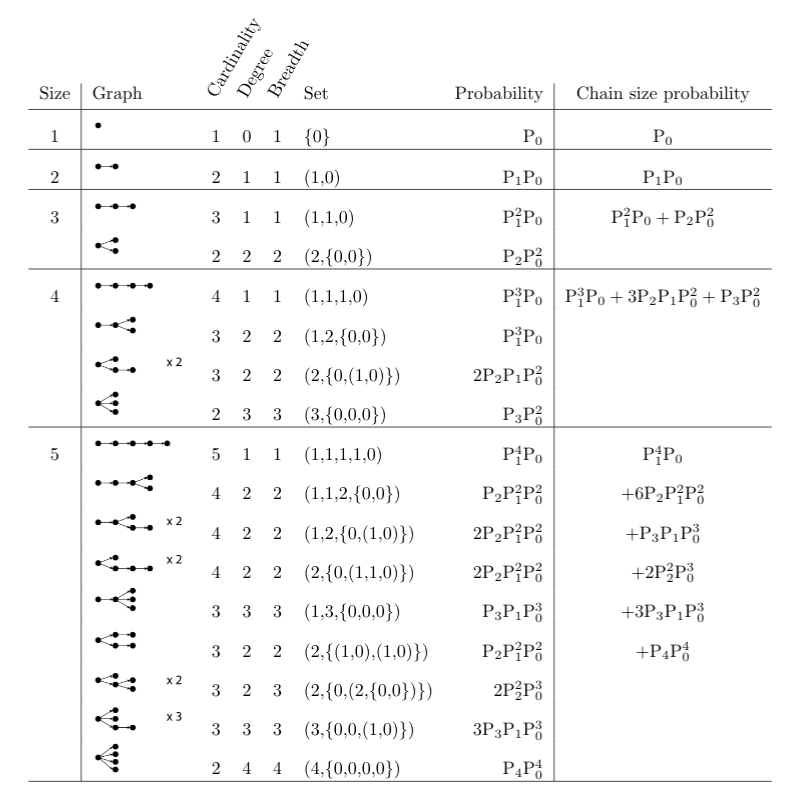
\includegraphics{Fig1.png}
    \caption{The possible ways of how outbreaks with a total of 1, 2, 3, 4 and 5 cases can arise, and their respective probabilities. }
    \label{fig:chainsdiagram}
\end{figure}
%Next we outline how to find the derivatives of $G(s)^y$.%before then outlining them for our problem

The derivatives of $Q(s) = (G(s))^y$ can be found using the chain rule for differentiation. The $n^{th}$ derivative of the inner function $g(s) = G(s)$ evaluated at $s=0$ is
\begin{equation}\label{eqn:g}
    g^{(n)}=  G^{(n)}(s)  \Bigr|_{s=0}
\end{equation}
and the $n^{th}$ derivative of the outer function $f(g(s))$ evaluated at $s=0$ is
\begin{equation}\label{eqn:f}
    f^{(n)}= \frac{y!}{(y-n)!} [G(s)]^{y-n}  \Bigr|_{s=0}.
\end{equation}
According to Faa di Bruno's formula \citep{Johnson2002-nq}, the $(y-1)^{th}$ derivative of $Q(s)$ evaluated at $s=0$ is
%give standard form first, then sum up in terms of Bell polys
\begin{equation}\label{eqn:fdb}
    \frac{d^{y-1} Q(s)}{ds^{y-1}} \Bigr|_{s=0} = \sum  f^{(n)} \frac{(y-1)!}{m_1! m_2! \dots m_{y-1}!} \left ( \frac{g'}{1!}\right )^{m_1} \left ( \frac{g''}{2!} \right )^{m_2}\dots \left ( \frac{g^{(y-1)}}{(y-1)!} \right )^{m_{y-1}}
\end{equation}
where the sum is over different solutions in non-negative integers $m_1, m_2, \dots, m_{y-1}$ of
\begin{align*}
    1. m_1 + 2. m_2 + \dots + (y-1) m_{y-1} &= y-1,\\
     m_1 + m_2 + \dots + m_{y-1} &= n.
\end{align*}
Equation \eqref{eqn:fdb} can be more succinctly written in terms of exponential Bell polynomials \citep{Johnson2002-nq, Cvijovic2011-ml}, which group the terms satisfying $m_1 + m_2 + \dots + m_{y-1} = n$ together,
\begin{equation}\label{eqn:fdbbell}
    \frac{d^{y-1} Q(s)}{ds^{y-1}} \Bigr|_{s=0} = \sum_{n=1}^{y-1}  f^{(n)}(g(s)) B_{y-1,n}(g'(s), g''(s), \dots, g^{(y-n)}(s))
\end{equation}
where $B_{y-1,n}(g', g'', \dots, g^{(y-n)})$ are Bell polynomials of the derivatives of the inner function. Numerous programs can compute the Bell polynomials of the derivatives, provided a formula for the inner function derivative is supplied, e.g., the BellB package in R \citep{??} and the BellY function in Mathematica.

Finally we note that by definition of the probability generating function for the $a_is$ we can write down the following in terms of probabilities,
\begin{align}\label{eqn:p0}
   G(0) =  P(A=0) &= p_0 \notag \\
    &=> f^{(n)}= \frac{y!}{(y-n)!} p_0^{y-n} 
\end{align}
and
\begin{align}\label{eqn:pn}
    P(A_i=n) &= \frac{1}{n!} G^{(n)}(s)\Bigr|_{s=0} \notag \\
    &=> n! p_n = G^{(n)}(s)\Bigr|_{s=0}.
\end{align}
Equations \eqref{eqn:g}, \eqref{eqn:f} and \eqref{eqn:fdbbell} together with \eqref{eqn:p0} and \eqref{eqn:pn} can be used to compute the chain size distribution numerically, which is particularly advantageous when an analytical formula for the chain size distribution cannot be readily obtained. The advantage of using the above equations is that it can used with any probability generating function $G(s)$, provided $G(s)$ is a composition of differentiable functions $f$ and $g$ with a sufficient number of derivatives. Additionally, it can compute the chain size distribution arising from an offspring distribution that is a weighted sum of probability generating functions such as equation \eqref{eqn:nbinommixpgf}. 

%now write in terms of probabilities and explain how the algorithm works, ie make a vector of g_s and combine with the fs according to the fdb formula
%disadvantage: brute force; cannot deal with large chains bigger than 30, but it can deal with any form of G, including when G is a mixture. 
\subsection{Chain size distribution for the negative binomial mixture}

To derive the chain size distribution for the negative binomial mixture, we use the result from \citet{Blumberg2013-xv} and therefore require the derivatives of powers of the generating function \eqref{eqn:nbinommixpgf}. Let $$T_y(s) =  (G_N(s))^y, \quad y = 1, 2, \dots $$ Then the probability of a chain having size $y$ \citep{Dwass1969-gs, Blumberg2013-xv} is
\begin{equation}\label{eqn:cluster}
    P(Y = y)  =\frac{1}{y}\left( \frac{1}{(y-1)!}T_y^{(y-1)}(s) \Bigr|_{s=0} \right ) =  \frac{1}{y!}T_y^{(y-1)}(s) \Bigr|_{s=0}
\end{equation}
To evaluate the derivatives of 
\begin{equation}\label{eqn:Qy}
   T_y(s)=  \left (\frac{p}{(1 + \frac{R_0^S}{k}(1-s))^k} +   \frac{(1-p)}{(1 + \frac{R_0^R}{k}(1-s))^k} \right)^y,
\end{equation}
we need to apply the chain rule for derivatives $y-1$ times.
The $n^{th}$ derivative of the inner function $g^{(n)}$ of equation \eqref{eqn:Qy},  $n = 1, 2, \dots, y-1$, evaluated at $s=0$ is
\begin{equation*}
    g^{(n)}(0) =  p \frac{(R_0^S)^n}{k^{n-1}} \displaystyle \prod_{i=1}^{n-1} (k+i) \left(1+\frac{R_0^S}{k}\right)^{-k-n}+ (1-p)\frac{(R_0^R)^n}{k^{n-1}} \displaystyle \prod_{i=1}^{n-1} (k+i)\left (1+\frac{R_0^R}{k}\right)^{-k-n}.
\end{equation*}
The $n^{th}$ derivative of the outer function $f^{(n)}$ of equation \eqref{eqn:Qy} evaluated at $s=0$ is
\begin{equation*}
    f^{(n)}(0) =  \frac{y!}{(y-n)! }\left (\frac{p}{(1 + \frac{R_0^S}{k})^k} +   \frac{(1-p)}{(1 + \frac{R_0^R}{k})^k} \right )^{y-n}, \quad n = 1, 2, \dots, y-1.
\end{equation*}
We substitute these formulas into the Faa di Bruno formula \eqref{eqn:fdbbell} and compute the chain size distribution \eqref{eqn:cluster} arising from the negative binomial mixture offspring distribution numerically using the BellB  software package in R \citep{??}.

%note what is not plotted here: major outbreaks.

%To examine the influence of having two contact processes with different intensities in the mixture model compared with having just one on the probability distribution, we compare the probability mass functions of the the mixture model \eqref{eqn:nbinommixpmf} with the standard model with same $R_0$ and dispersion parameter $k$ in Figure \ref{fig:pmf}. The probability of an infectious individual producing no secondary infections ($P(N=0)$) is higher in the mixture models than the base model for all values of $k$. As $k$ increases, the level of heterogeneity declines in that $P(N=0)$ declines in both models, but the standard model has a greater central tendency than the mixture model. In sum, there are visible differences in the probability mass functions of both models, and we conclude that having a mixture of two contact processes substantially affects the probability mass function. 


%In Figure \ref{fig:chains} we compare the chain size distributions of the mixture model ($R_0^R=1.1$, $p=0.1$, additional contacts $\delta =9$) with the standard model for $R_0>1$ and various values of $k$. The mean number of secondary infections for both models is $R_0 =2$. The mixture model chain size distribution is characterized by greater probabilities of observing small chains that go extinct (i.e., transmission chains consisting of less than 10 secondary infections) than the standard model. Assuming there is population structure in a dataset and $R_0>1$, we would expect to see more small chains compared to a dataset where there is no structuring in contact. For example, if $R_0=2$ and $k=2$, the mixture model predicts 64\% of transmission chains will be small. On the other hand, the standard model predicts just 38\% of infection clusters will be small, and the remainder will be major outbreaks (e.g., Figure \ref{fig:compcdf}). Figure \ref{fig:compcdf} shows there is a steep decline in the proportion of chains greater than a specified outbreak size between outbreak sizes of 1 and 20, and the drop-off is more pronounced for the mixture models than the standard models. This is because the probability of no secondary infections is larger for the the mixture model than the standard model \citep{Garske}. In sum, the chain size distribution, given a dataset consisting of small and major infection clusters, would look substantially different if there is underlying population structure in contact rates compared to one without. %something of interest - this isnt observed when R0<1...the base model has higher probs of small chains than the mixture model.

%also the R0<1 case has relevance for control. 

%should i show the converging to the major outbreak for each value of k? and how it is substantially different for each value of k




%Derivation
%Figure 2: comparison of chain size distributions for standard and mixture models for various values of $k$
%summary statistics for transmission chains - can use the distirubion to calculate the cumulative probability of observing a small chain
%mean chain size conditioned on extinction 
%variance of chain size conditioned on extinction 

%where does control activities thresholds go?
%what journal to target??

\subsection{Chain size distribution statistics}

To study the characteristics of the chain size distribution for $R_0>1$, using equation \eqref{eqn:R0star} we numerically calculate the mean chain size conditioned on extinction \citep{Yan2008-jc}, 
\begin{equation}\label{eqn:meanchain}
   E(Y|\text{minor outbreak}) = m_c= \frac{1}{1-R_0^*},
\end{equation}
and the variance of chain sizes conditioned on extinction,
\begin{equation}\label{eqn:varchain}
    V(Y|\text{minor outbreak}) =v_c = \frac{s^* G_N''(s^*)+R_0^{*}(1-R_0^*)}{(1-R_0^*)^3}
\end{equation}
Using equation \eqref{eqn:cluster}, we also compute the proportion of chains greater than size $y$ (i.e., the area under the tail of the chain size distribution) by numerically calculating the complementary cumulative distribution function for $y = 1, 2,\dots,$
\begin{equation}
    P(Y>y) = 1-P(Y\leq y). 
\end{equation}

% As $R_0$ increases, the probability of a minor outbreak $z_\infty$ declines. Therefore $R_0^*$ declines with $R_0$, and so the mean chain size will also decline (Figure \ref{fig:meanchain}). For example, for the baseline Poisson model, $R_0^*= G'(z_\infty) = R_0 e^{(R_0(z_\infty -1 ))}$, which decreases as $z_\infty$ decreases.

\subsection{Numerical study of summary statistics}

Hallmarks of superspreading include  high probability of observing no secondary infections per infected individual, high variability in the number of secondary infections per infected individual, small probability of major epidemics, high variability in transmission chain sizes, and high probability of observing small transmission chains. Unlike the standard negative binomial model, the mixture model \eqref{eqn:nbinommixpmf} assumed the population can be grouped by contact rate. We would like to understand how this affects the stochastic characteristics of transmission chains. To compare stochastic characteristics of the standard negative binomial model and finite mixture negative binomial model, we calculated four summary statistics. To assess differences in variability in cases in both models, we used the coefficient of variation of the number of secondary infections. To compare the chain size distributions arising from both models, we numerically calculated the probability of a major outbreak, and the mean and coefficient of variation of minor outbreaks. 

To calculate the summary statistics, we ensured that the basic reproduction number $R_0$ and the dispersion parameter $k$ were the same for each comparison of the standard and mixture models. We set $R_0=2$ for all models studied. To explore the impact of variability in infectious period distributions in output from the standard and mixture models, we varied the dispersion parameter $k$ between $1/2$ and $4$. To study the effect of the proportion of superspreaders in the population on outbreaks,  we varied $p$ and $\delta$ in the mixture model while keeping the basic reproduction number fixed at $R_0 = R_0^R + p \delta = 2$. As $p$ is increased, the number of additional contacts $\delta$ must be reduced to keep $R_0$ fixed at 2, i.e., a superspreading cohort that forms a low proportion of the overall population must have a high additional contact rate over the average infectious period. We varied the superspreading proportion $p$  between $0.01$ and $1$ while simultaneously adjusting the number of additional contacts $\delta = (R_0 -R_0^R)/p$ with regular basic reproduction number $R_0^R$ fixed at 1.1 to retain $R_0$ at 2.  All statistics were calculated using R 4.1.1 and code is supplied in XX. 

%should I include chain size of 1 as a stat (chain size distrib depends on this)

\section{Comparison of mixture model with standard model}

%How does the addition of population structure affect stochastic characteristics at the beginning of an outbreak? Do they differ those arising from the standard model?

\subsection{Comparison of probability mass functions}

%%Parameter tables here

To examine the influence of having two contact processes with different intensities in the mixture model compared with having just one on the probability distribution, we compare the probability mass functions of the mixture model \eqref{eqn:nbinommixpmf} with the standard model with same $R_0$ and various values of dispersion parameter $k$ in Figure \ref{fig:pmf}. The probability of an infectious individual producing no secondary infections ($P(N=0)$) is higher in the mixture models than the standard model for all values of $k$. As $k$ increases, the level of heterogeneity declines in that $P(N=0)$ declines in both models, but the standard model has a greater central tendency than the mixture model. In sum, there are visible differences in the probability mass functions of both models, and we conclude that having a mixture of two contact processes substantially affects the probability mass function. 

\begin{figure}%[!t] %F1
\centering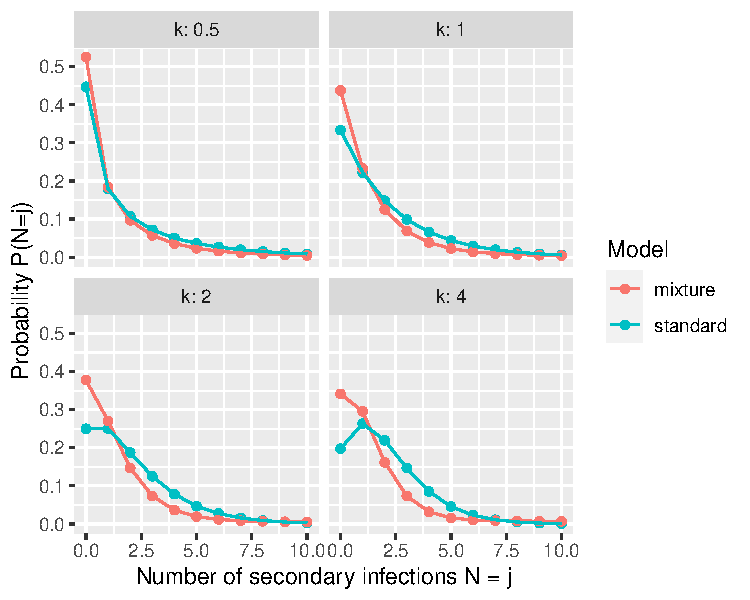
\includegraphics {Figure1.pdf}
\caption{Probability mass functions of the mixture model ($R_0^R=1.1$, $p=0.1$, additional contacts $\delta =9$) compared with those of standard model with the same $R_0$ and dispersion parameter $k$. The mean number of secondary infections for both models is $R_0 =2$. For the mixture models, the probability of no secondary infections is always greater than the negative binomial model with the same $R_0$ and $k$. As $k$ increases there is a greater central tendency in the number of secondary infections in the standard model.  }
\label{fig:pmf}\vspace*{-9pt}
\end{figure}

\subsection{Comparison of chain size distributions}



In Figure \ref{fig:chains} we compare the chain size distributions of the mixture model ($R_0^R=1.1$, $p=0.1$, additional contacts $\delta =9$) with the standard model for various values of $k$. These chain size distributions result from the offspring distributions shown in Figure \ref{fig:pmf}. The mean number of secondary infections for both models is $R_0 =2$. The larger probability of singular chains in the mixture models is balanced by higher frequencies of small outbreaks consisting of 2, 3, 4, $\dots$ cases, which is particularly pronounced for larger dispersion values $k$. The mixture model chain size distributions are characterized by greater probabilities of observing small outbreaks that go extinct (i.e., transmission chains consisting of less than 10 secondary infections) than the standard model. For example, the probability of observing a chain size of two, $p_1 p_0$, is greater for the mixture model than the standard model if $R_0 > 1$. This result suggests that assuming there is population structure in a dataset and $R_0>1$, we would expect to see higher frequencies of small chains compared to a dataset where there is no structuring in contact. %we note this is not observed when R0 < 1

%explore this more closely in figure 3 - need to read Garske
%the difference is more clearly captured by studying the tails
%Next we show that the tail of the distribution has very different properties for the mixture vs the standard model
The difference between the chain size distributions generated by the standard and mixture models is more clearly captured by studying the tails of the chain size distributions in  Figure \ref{fig:compcdf}. The proportion of outbreaks greater than size $y$  converge to the probability of a major outbreak $1-s^*$ for large chain sizes $y$ (horizontal lines in each figure). There is a substantial difference in the predicted frequency of large clusters for the standard and mixture models.
For example, if $R_0=2$ and $k=2$, the mixture model predicts 36\% of transmission chains will be large (red horizontal line in  Figure \ref{fig:compcdf}c). On the other hand, the standard model predicts 62\% of infection clusters will be large (blue horizontal line in  Figure \ref{fig:compcdf}c), and the remainder will be small outbreaks (e.g., Figure \ref{fig:chains}c). Figure \ref{fig:compcdf} also shows there is a steep decline in the proportion of chains greater than a specified outbreak size between 1 and 20, and the drop-off is more pronounced for the mixture models than the standard models. This is because the probability of no secondary infections is larger for the mixture model than the standard model \citep{Garske2008-ax}.  In sum, these results suggest that the chain size distribution, given a dataset consisting of small and major infection clusters, would look substantially different if there is underlying population structure in contact rates compared to one without. %something of interest - this isnt observed when R0<1...the base model has higher probs of small chains than the mixture model.

%l

\begin{figure}
    \centering
    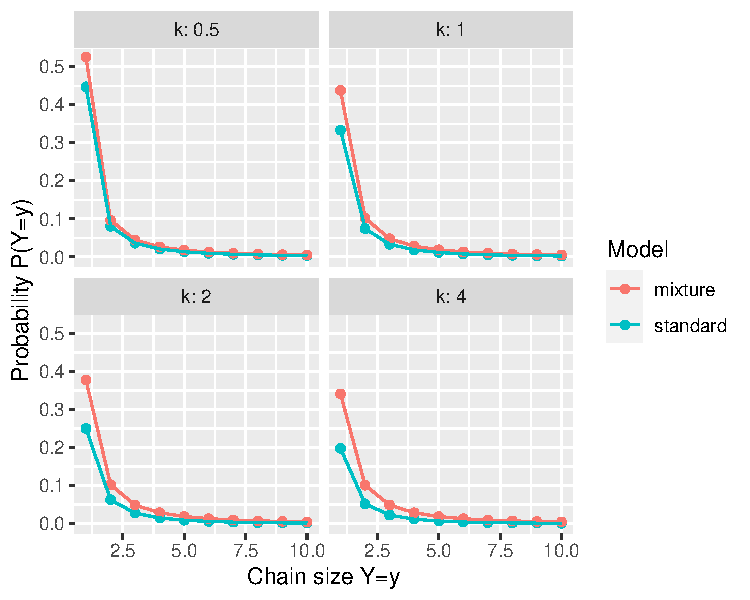
\includegraphics{Figure2.pdf}
    \caption{Chain size distributions of the mixture model ($R_0^R=1.1$, $p=0.1$, additional contacts $\delta =9$) compared with those of the standard model with the same $R_0$ and dispersion parameter $k=0.5, 1, 2, 4$. The mean number of secondary infections for both models is $R_0 =2$. For the mixture models, the probability of a chain size of one is always greater than the negative binomial model with the same $R_0$ and $k$.  The chain size distribution is longer tailed for the mixture models compared to the corresponding standard models. }
    \label{fig:chains}
\end{figure}

\begin{figure}
    \centering
    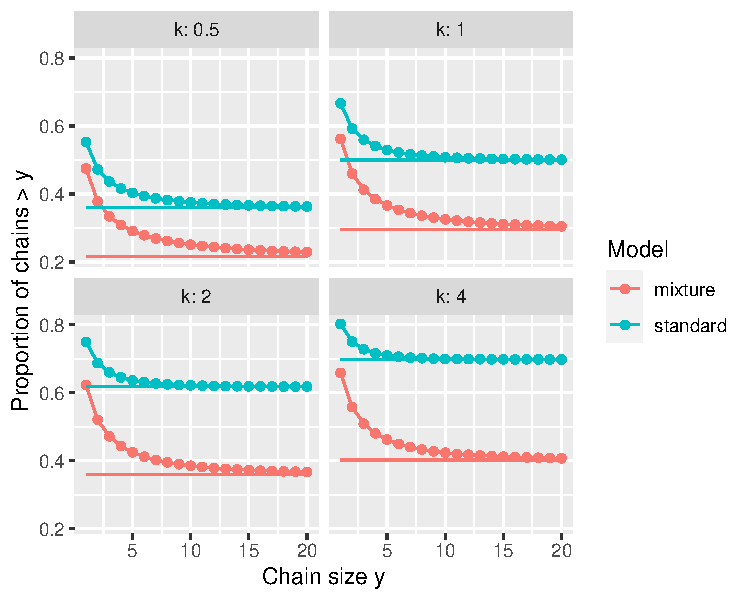
\includegraphics{Figure3.pdf}
    \caption{The proportion of outbreaks bigger than size $y$ is the area under the tail of the chain size distribution $P(Y>y)$ arising from the standard negative binomial model (red) and the mixture model (blue). For large chain sizes the curves converge to the probability of a major outbreak, $1-s^*$. Horizontal lines indicate the probability of a major epidemic arising from each branching process.}
    \label{fig:compcdf}
\end{figure}

We note that the dispersion parameter $k$ does not have to less than one for extreme heterogeneity in transmission to arise via the mixture model. For example, Table \ref{tab:summary} shows that the coefficient of variation of secondary infections arising from a mixture model with 10\% of individuals belonging to the superspreader cohort with $R_0^S=10.1$, 90\% belonging to the regular cohort with $R_0^R=1.1$ and a dispersion parameter of 2 is 93\% higher than that arising from a standard model with $R_0=2$ and $k=2$. The higher variance in the number of secondary infections induces higher probability that a chain contains a single case and greater variability in minor outbreak sizes (e.g., the coefficient of variation of the chain sizes is 46\% higher than those obtained from the standard model). Major outbreaks in the mixture model are 42\% less likely and the mean size of small outbreaks is 39\% greater than the standard model. In the next section we explore summary statistics across a range of values for the fraction of superspreaders $p$ and dispersion parameter $k$. 

\begin{table}[h!] %T2
\tblcaptionnotes{Comparing summary statistics for mixture and standard model for $R_0=2$, $k=2$, $p=0.1$, $\delta =9$, $R_0^R=1.1$}
{\mbox{\tabcolsep=10pt\begin{tabular}{@{}ccccccc@{}}
\tblhead{model & $P(Y=1)$ & $V(N)$  &  $\sqrt{V(N)}/R_0$ & $1-s^*$ & $m_c$  & $\sqrt{v_c}/{m_c}$ \\[-11pt]}\\[-9.5pt]
 standard    & 0.2500000    & 4.000     & 1.000000 &    0.6180314 & 1.894435 &1.051468 \\[3pt]
 mixture   &  0.3773418 &   14.935   &    1.932291    & 0.3608386 & 2.631973& 1.535524
  \\[-9pt] \lastline
\end{tabular}
\label{tab:summary}
}}{}\vspace*{-2pt}%leave footnote space blank, e.g. $^a$ Iteration counts obtained with the ideal preconditioner are
%listed in columns 2--3 of Table 2\\$^b$ The negative eigenvalues
%of the preconditioned saddle point system.
\end{table}




\subsection{Summary statistics study} %results of summary stats study

%Hallmarks of superspreading include  high probability of observing no secondary infections per infected individual, high variability in the number of secondary infections per infected individual, small probability of major epidemics, high variability in transmission chain sizes, and high probability of observing small transmission chains. Unlike the standard negative binomial model, the mixture model \eqref{eqn:nbinommixpmf} assumed the population can be grouped by contact rate. We would like to understand how this affects the stochastic characteristics of transmission chains. To compare stochastic characteristics of the standard negative binomial model and finite mixture negative binomial model, we calculated four summary statistics. To assess differences in variability in cases in both models, we used the coefficient of variation of the number of secondary infections. To compare the chain size distributions arising from both models, we numerically calculated the probability of a major outbreak, and the mean and coefficient of variation of minor outbreaks. 

%To calculate the summary statistics, we ensured that the basic reproduction number $R_0$ and the dispersion parameter $k$ were the same for each comparison of the standard and mixture models. We set $R_0=2$ for all models studied. To explore the impact of variability in infectious period distributions in output from the standard and mixture models, we varied the dispersion parameter $k$ between $1/2$ and $4$. To study the effect of the proportion of superspreaders in the population on outbreaks,  we varied $p$ and $\delta$ in the mixture model while keeping the basic reproduction number fixed at $R_0 = R_0^R + p \delta = 2$. As $p$ is increased, the number of additional contacts must be reduced to keep $R_0$ fixed at 2, i.e., a superspreading cohort that is a low proportion of the overall population must have a high additional contact rate over the average infectious period. We varied the superspreading proportion $p$  between $0.01$ and $1$ while simultaneously adjusting the number of additional contacts $\delta = (R_0 -R_0^R)/p$ with regular basic reproduction number $R_0^R$ fixed at 1.1 to retain $R_0$ at 2.  All statistics were calculated using R 4.1.1 and code is supplied in XX. 



%move to discussion Statistics generated using the mixture model \eqref{eqn:nbinommixpmf} differ substantially from those generated using the standard model if the population consists of a low proportion of superspreaders (Figures 4-7). Taken together, these results suggest that comparing across different heterogeneous population combinations with the same $R_0$ and $k$ leads to very different outbreak dynamics than those obtained from the baseline model, and these outbreaks are characterized by higher probabilities of observing a chain that extinguishes quickly and greater variability in the sizes of minor outbreaks.

 A measure of variability of cases generated per individual is the coefficient of variation of secondary infections.  Figure \ref{fig:CVcases} shows the coefficient of variation for the mixture and standard models for $R_0=2$ and various values of dispersion parameter $k$ as the fraction of superspreaders $p$ is varied. High variability in the mixture offspring distribution is predicted for all values of $k$ provided the average number of additional contacts $\delta$ is large (i.e., fraction of superspreaders $p$ is small). The coefficient of variation generated from the mixture model decreases with $p$ and converges to the corresponding value of the standard model with $R_0=2$ as $p\rightarrow 1$ ($\delta\rightarrow R_0-R_0^R$) because $p R_0^S+(1-p)R_0^R$ approaches $R_0^S = R_0$. The greatest disparity between the mixture model and standard model is for mixtures with small dispersion parameter $k$, small proportion of superspreaders $p$ and large average number of additional contacts $\delta$. 
 
 \begin{figure}
    \centering
    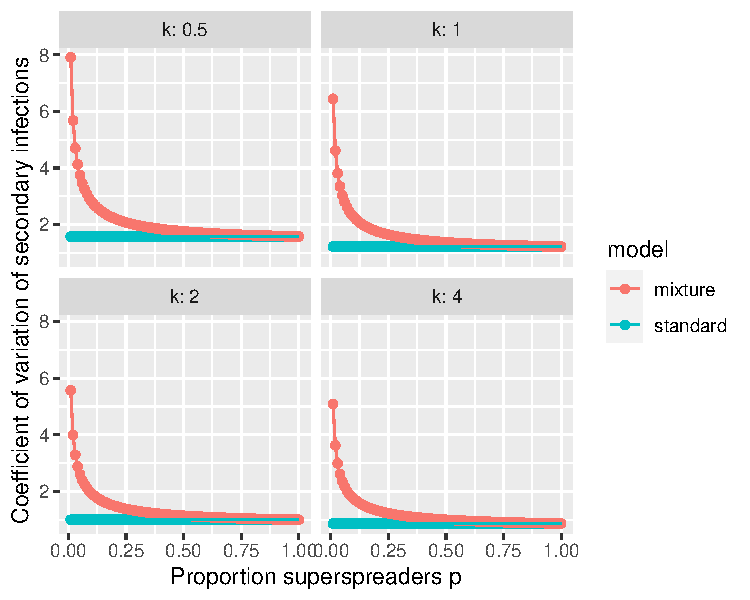
\includegraphics{Figure4.pdf}
    \caption{Coefficient of variation of secondary infections in the mixture model is highest for small dispersion parameter $k$, small $p$ and large number of additional contacts $\delta$. The coefficient of variation of secondary infections in the mixture model decreases as $p$ increases and approaches the value of the standard model as $p$ approaches 1. There is greater variability in the number of secondary infections in the mixture model compared to the standard model, even if $k>1$, with the highest variability for small dispersion parameter $k$, small $p$ and large number of additional contacts.  }
    \label{fig:CVcases}
\end{figure}

 
 The pattern in variability of secondary infections drives the behavior of the coefficient of variation in chain sizes (Figure \ref{fig:CVchain}), with chain size distributions generated by mixtures exhibiting high variability for large $\delta$,  small $p$ and small $k$. However, Figure \ref{fig:meanchain} shows that the mean of chain sizes conditioned on extinction increases with dispersion parameter $k$, with the largest means for small $p$, large $\delta$ and large $k$, suggesting that infectious periods with a central tendency combined with heterogeneous contact patterns could generate sizeable transmission chains. 
 
 \begin{figure}
    \centering
    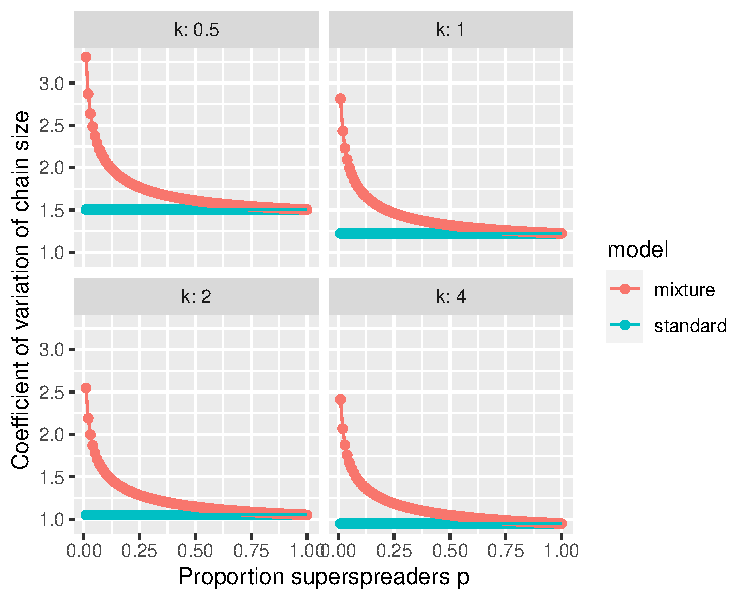
\includegraphics{Figure7.pdf}
    \caption{The coefficient of variation of transmission chain sizes in the mixture model is highest for small dispersion parameter $k$, small $p$ and large number of additional contacts $\delta$. The coefficient of variation of small chains that go extinct in the mixture model decreases as $p$ increases and approaches the value of the standard model as $p$ approaches 1. There is greater variability in chain sizes in the mixture model compared to the standard model, even if $k>1$, with the highest coefficients of variation observed for small dispersion parameter $k$, small $p$ and large number of additional contacts. }
    \label{fig:CVchain}
\end{figure}

\begin{figure}
    \centering
    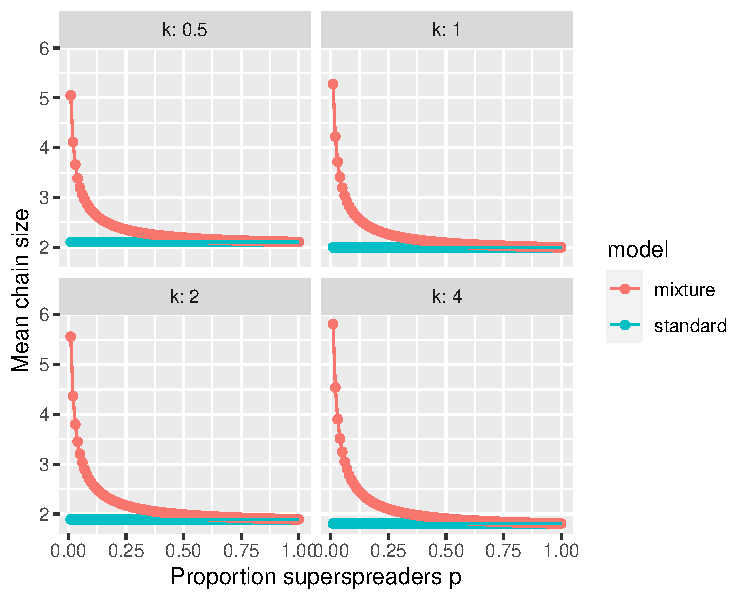
\includegraphics{Figure6.pdf}
    \caption{Mean chain sizes are largest for large dispersion parameter $k$, small $p$ and large number of additional contacts $\delta$. Mean chain sizes decrease as $p$ increases and approaches the value of the standard model as $p$ approaches 1. Mean chain sizes are larger in mixture models compared to the standard model, even if $k>1$. }
    \label{fig:meanchain}
\end{figure}

 
  In Figure \ref{fig:outbreak}, the probability of a major epidemic increases with $p$ and $k$, converging to the value predicted by the standard model as $p$ approaches 1, with the lowest values occurring for small $k$ and small $p$ (large $R_0^S$). The biggest disparity in predictions for frequency of large clusters between the mixture and standard model occurs for $k=4$. The mixture model with small $p$ and large $\delta$ retains low probability of large clusters, a hallmark of superspreading,  unlike  the corresponding standard model.
  
  \begin{figure}
    \centering
    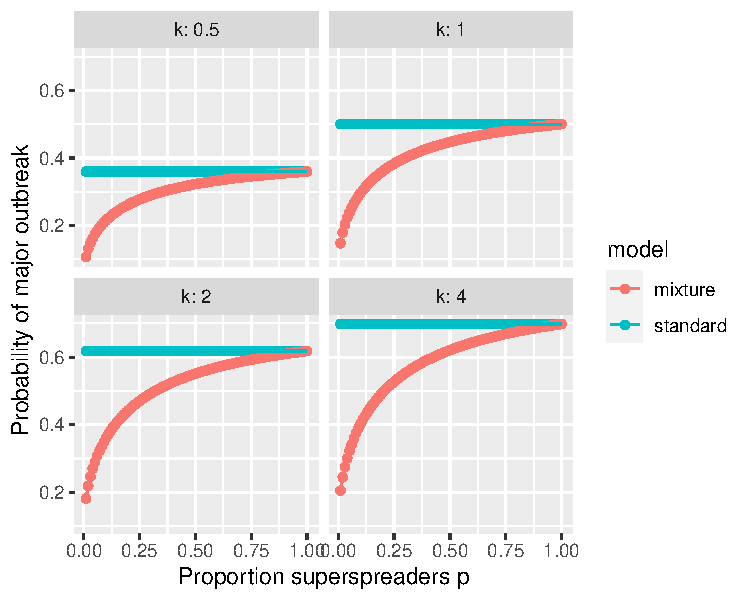
\includegraphics{Figure5.pdf}
    \caption{ Probability of a major outbreak in the mixture model is lowest for small dispersion parameter $k$, small $p$ and large number of additional contacts $\delta$. The probability of a major outbreak in the mixture model increases as $p$ increases and approaches the value of the standard model as $p$ approaches 1. There is smaller probability of major epidemics in the mixture model compared to the standard model, even if $k>1$, with the lowest probabilities for small dispersion parameter $k$, small $p$ and large number of additional contacts.}
    \label{fig:outbreak}
\end{figure}
  
  Taken together, the results in Figures 4-8 suggest that comparing across different heterogeneous population combinations with the same $R_0$ and $k$ leads to very different outbreak dynamics than those obtained from the standard model, and these outbreaks are characterized by higher probabilities of observing minor outbreaks and greater variability in the sizes of small transmission chains.
  
  %biggest disparity between k=4 (STANDARD) and small p mixture
  %THE POINT IS K>1 HETEROGENEOUS OUTBREAKS WITH CHARACTERISTICS OF SUPERSPREADING AND HIGHER MEAN CHAIN SIZE
  %extend the table to all values of k??
  
  
  %All of these statistics decrease with $p$ and converge to the corresponding value of the standard model with $R_0=2$ as $p\rightarrow 1$ ($\delta\rightarrow R_0-R_0^R$) because $p R_0^S+(1-p)R_0^R$ approaches $R_0^S = R_0$. 
  
 
 %%paragraph on probability of major outbreak
 
 %mean chain size conditioned on extinction (ie minor outbreaks - mean chain size is largest for large k
 
 
 
 %%CV of chains
 
 %% mean of chains conditioned on extinction
 
 

%influence of variability in cases

%shouldt this go before or after the figures?
 %higher mean chain size and probability that a chain contains a single case
%need a concluding sentence

%The mean chain size and coefficients of variation of cases and chain sizes generated from the mixture model are highest for low proportions of superspreaders  and smaller values of the dispersion parameter. All of these statistics decrease with $p$ and converge to the corresponding value of the standard model with $R_0=2$ as $p\rightarrow 1$ ($\delta\rightarrow R_0-R_0^R$) because $p R_0^S+(1-p)R_0^R$ approaches $R_0^S = R_0$. In Figure 7, the probability of a major epidemic increases with $p$, with the lowest values occurring for small $k$ and small $p$ (large $R_0^S$). Taken together, these results suggest that comparing across different heterogeneous population combinations with the same $R_0$ and $k$ leads to very different outbreak dynamics than those obtained from the baseline model, and these outbreaks are characterized by higher probabilities of observing a chain that extinguishes quickly and greater variability in the sizes of minor outbreaks. 


%properties of chain size distribution: mean, CV, frequency of large clusters


\section{Control activities}

 %What features should be targeted that would control an epidemic? Which strategy would lead to the greatest reduction in the probability of a major epidemic? How do control strategies affect case variability? %reduction in cases?
%\subsection{Numerical analysis} %studies (assuming $R_0$ > 1)
%How statistics vary with $p$, $\delta$ and $k$, keeping $R_0$ fixed, for the baseline and mixture models (compare the degree of heterogeneity in outbreak patterns)
%Effect of control activities on outbreak patterns: decrease $R_0^R$, $p$ and $\delta$ by factor $1-c$ and study their effect on variance to mean ratio and probability of extinction (which control activity induces greatest probability of extinction for a given level of control effort below the threshold (assuming the threshold for all activities is the same) and do patterns become more heterogeneous as epidemic control is applied?)

How do we control superspreading in a heterogeneous population? Control efforts can either target superspreaders alone, or they can be focused towards both superspreading and regular cohorts. Here we will study the effect of three ways of reducing the basic reproduction number $R_0$:
\begin{itemize}
\item[(a)] decreasing the proportion $p$ of individuals in the population with high contact rate, which may
be considered to be the same as increasing the proportion of the population that become vaccinated or increasing the proportion of the population who respond to information about disease risk through an education campaign; %self-isolate when sick or comply with
%stay-at-home orders/physical distancing, comply with face covering mandates or other measures that reduce the chance of transmission;
\item [(b)] decreasing the number of additional contacts per individual $\tilde{\delta}$ in the superspreading cohort, e.g., this group practises self-isolation when symptomatic;
\item [(c)] decreasing baseline transmission rate in both groups by reducing $R_0^R$, e.g., both groups wear face coverings, practise social distancing or mix in a well-ventilated environment. 
\end{itemize}
Strategies (a) and (b) are aimed towards reducing the degree of superspreading, and are similar to the targeted individual control policies suggested in \citet{Lloyd-Smith2005-ma}. Strategy (c) focuses decreasing transmission in both cohorts and is therefore a population-wide control policy \citep{Lloyd-Smith2005-ma}.. For each strategy, we calculate the critical control effort threshold for elimination, i.e., the level of effort required for the probability of a major epidemic to be zero. We ask which of these strategies leads to the fastest reduction in the probability of a major epidemic for the least level of effort, assuming that the critical threshold for elimination is the same for all activities. 

\subsection{Critical thresholds for elimination}

We firstly study the effect of targeted control activities on the superspreading cohort. We denote control effort by $c$, $0\leq c\leq 1$, where $c=0$ implies the application of no control effort and $c=1$ indicates full control of  transmission. We firstly alter population structure by reducing $p$ (thereby increasing $1-p$) by a factor $1-c$ while keeping all other parameters fixed. Secondly, we reduce the individual reproduction number by decreasing the number of additional contacts over the course of an average infectious period $\delta$ by a factor $1-c$ while keeping all other parameters fixed.  Strategies (a) and (b) have the same effective $R_0$,
\begin{equation}\label{eqn:effectiveR0S}
R_{0e}^{S} = R_0^R + (1-c) p \delta.
\end{equation}
When $c=1$, effective $R_0$ is the same as $R_0^R$, the basic reproduction number of the pathogen in the regular transmission cohort. If $R_0 > 1$, the threshold control effort for elimination when control is limited to the superspreading cohort is 
\begin{equation}\label{eqn:thresholdS}
c^{S} = 1 -\frac{ (1-R_0^R)}{p \delta}    = \frac{R_0-1}{p \delta} =\frac{R_0-1}{R_0-R_0^R}, \quad 0< c^{S} \leq 1.
\end{equation}
Therefore the pathogen can only be eliminated in the entire population if $R_0^R < 1$, i.e., the regular cohort cannot sustain the infection alone. 


We also study the effect of mitigation measures on both cohorts (strategy (c)), by reducing $R_0^R$ by a factor $1-c$. Strategy (c) has a different expression to strategies (a) and (b) for effective $R_0$,
\begin{equation}\label{eqn:effectiveR0SR}
R_{0e}^{SR} = (1-c) R_0^R + p \delta, 
\end{equation}
and consequently different expression for threshold control effort,
\begin{equation}\label{eqn:thresholdSR}
c^{SR} = 1 -\frac{ (1-p \delta)}{R_0^R} = \frac{R_0-1}{R_0^R}, \quad 0 < c^{SR} \leq 1.
\end{equation}
In this case, if $c=1$, then $R_{0e}^{SR} = p \delta$, and elimination of the disease in the entire population can only be achieved provided $p \delta = R_0 - R_0^R < 1$, i.e., the superspreading cohort cannot have too many additional contacts, or the proportion of superspreaders in the population cannot be too large. 

The critical control thresholds  \eqref{eqn:thresholdS} and \eqref{eqn:thresholdSR} are equal if and only if $R_0 = 2 R_0^R$, or equivalently $R_0^R = p \delta$. If $R_0< 2 R_0^R$ (i.e., $p\delta <R_0^R$) then $c^{SR}<c^{S}$ and targeting control activities towards both groups leads to a lower threshold for elimination. On the other hand, if $R_0>2R_0^R$ (i.e., $p \delta > R_0^R$) then $c^{S}< c^{SR}$ and targeting control activities towards the superspreading cohort only induces more efficient elimination. %is a more efficient strategy

Comparing the effective reproduction numbers \eqref{eqn:effectiveR0S} and \eqref{eqn:effectiveR0SR}, if $p \delta < R_0^R$ (i.e., superspreaders contribute little to $R_0$), use of control activities that target both groups is a more effective strategy than targeting superspreaders alone since $R_{0e}^{SC} < R_{0e}^{S}$.   On the other hand, if $p\delta > R_0^R$, $R_{0e}^{S} < R_{0e}^{SC}$ and so targeting superspreading leads to a greater reduction in $R_0$ than targeting both groups with control. 

%context dependent
\subsection{Variance to mean ratio}

To study how control activities impact heterogeneity in outbreak patterns, we examine the variance to mean ratio of the number of secondary infections. We expect that if control efforts focus on actions that reduce $p$ or $\delta$, heterogeneity in outbreaks should decline with the level of control effort because the sources of heterogeneity and superspreading are being directly targeted. On the other hand, if both groups are subject to control activity with regular transmission $R_0^R$ being targeted (and therefore $R_0^A=R_0^R + \delta$ also being targeted), the influence of superspreaders may dominate outbreak patterns. For example, at $c=1$, if superspreading only is targeted, the variance to mean ratio is $1+R_0^R/k$ whereas if both groups are simultaneously targeted, it is $1+\delta/k + \delta(1-p)$. In the full control scenario, if $\delta > R_0^R$ then the variance to mean ratio for control applied to both groups is larger than that for superspreading only, whereas if $\delta$ is very small, the variance to mean ratio for both group control is close to unity. 

%note this is not the only way...this is just a numerical example. Will get difference answers depending on the critical threshold for each strategy..
%To answer the question of how the three control activities of interest affect outbreak patterns as epidemic control $c$ is applied, we would like the threshold for extinction to be the same for all activities, and therefore effective $R_0$ declines at the same rate.
\subsection{Numerical case study}

Our analytical results indicate that elimination of disease under each control activity is only possible in certain circumstances. As a case study, we assume elimination is achievable for all activities and then compare outcomes of the three strategies.  To assess how case variability and the probability of a major outbreak change with each control strategy, we choose parameters such that the threshold for extinction is the same for all activities, and therefore effective $R_0$ declines at the same rate. We start with $R_0^R = 0.9 <1$, which guarantees extinction for targeted control because the threshold will be less than one. We choose $R_0 = 2 R_0^R = 1.8$, which means that $p \delta = 0.9 <1$, so extinction will be guaranteed if control to both groups is applied. We choose $p = 0.1$ and $\delta = 9$. In this scenario, effective $R_0$ (equations \eqref{eqn:effectiveR0S} and \eqref{eqn:effectiveR0SR}) is the same for all three strategies. Then we decrease each of $R_0^R$, $p$ and $\delta$ by a factor $1-c$ in increments of 0.01 and examine their effect on the variance to mean ratio of secondary infections, the probability of extinction, and the percentage reduction in the probability of a major outbreak from the baseline at $c=0$.


Figures \ref{fig:extprob}-\ref{fig:varmeanratio} show that control strategies have different impacts on probability of extinction and variance to mean ratio as a function of control effort even when the threshold for extinction is the same for all three strategies ($c^S = c^{SR} = 8/9$). Control actions that act on both groups lead to greater heterogeneity in outbreaks (i.e., higher variance to mean ratio in secondary infections) than control measures that act on superspreaders only (e.g., reducing the number of additional contacts $\delta$ and reducing the proportion of superspreaders $p$). 

%the following percentages need to be checked
For low levels of control effort, Figure \ref{fig:percentchange} shows that targeting both groups reduces the probability of a major epidemic more efficiently than targeting superspreaders. For example, the chance of a major outbreak is reduced by 25\% if control aimed at both groups at 12.5\% effort is applied. The superspreading proportion would have to reduced by ~37.5\%, or the number of additional contacts made by superspreaders would have to be decreased by ~50\% to reduce the chance of a major outbreak by 25\%.  However, targeting both groups comes at a cost that the other control activities do not have: increased variability in the number of cases generated per person (Figure \ref{fig:varmeanratio}). On the other hand, we note that while reduction of contacts is the control activity that reduces heterogeneity in outbreaks the most, it is also the least effective in terms of reducing the chances of a major outbreak. Targeting the proportion of superspreaders offers the middle ground of together reducing the variance-to-mean ratio and the probability of a major outbreak with increasing control effort. %We note that these results depend on the scenario

%In conclusion, for high levels of control effort better to focus on targeting the superspreading cohort because it will also reduce heterogeneity in cases

%Want figures 8 and 9 to be a 2 panel plot. 
\begin{figure}
    \centering
    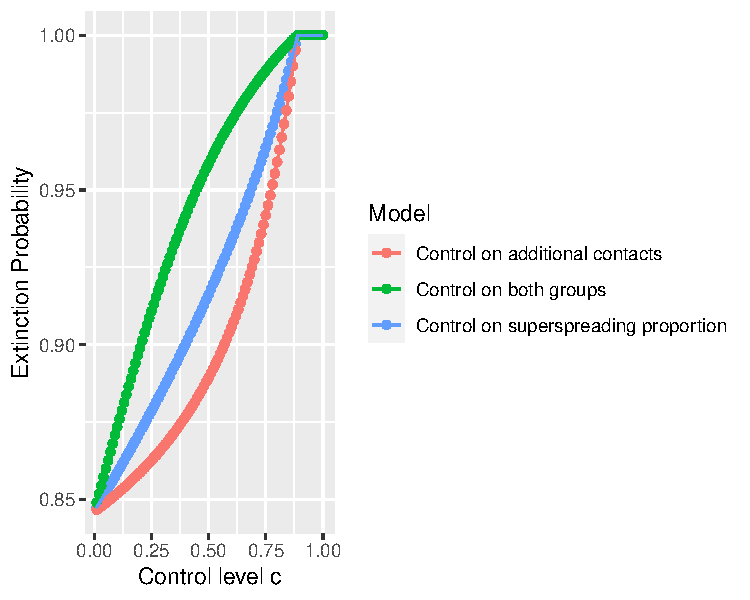
\includegraphics{Figure8.pdf}
    \caption{Panel a shows the extinction probability as a function of control level and panel b shows the corresponding percentage decrease in the probability of a major outbreak as the control level $c$ increases. Control applied to both groups activates the fastest increase in extinction probability and respective reduction in the probability of a major outbreak.  }
    \label{fig:extprob}
\end{figure}

\begin{figure}
    \centering
    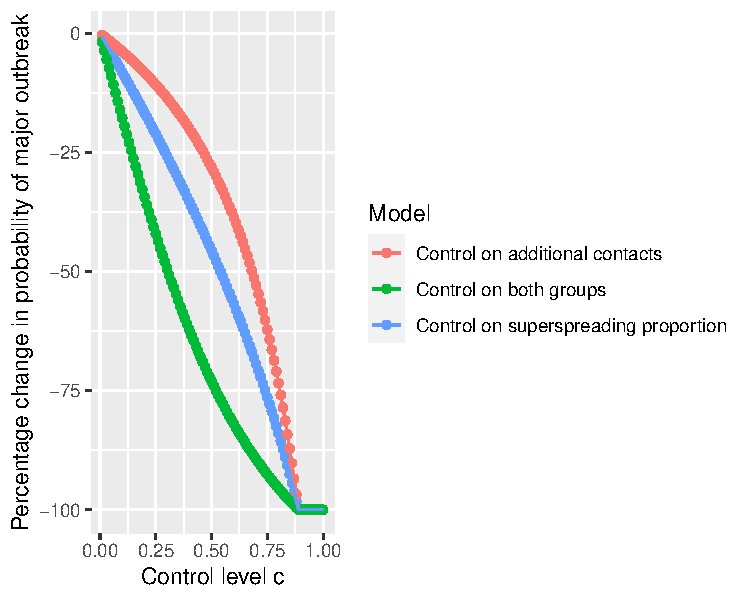
\includegraphics{Figure10.pdf}
    \caption{Control applied to both groups activates the fastest reduction in the probability of a major outbreak.}
    \label{fig:percentchange}
\end{figure}

%controlling both groups comes at a cost:
\begin{figure}
    \centering
    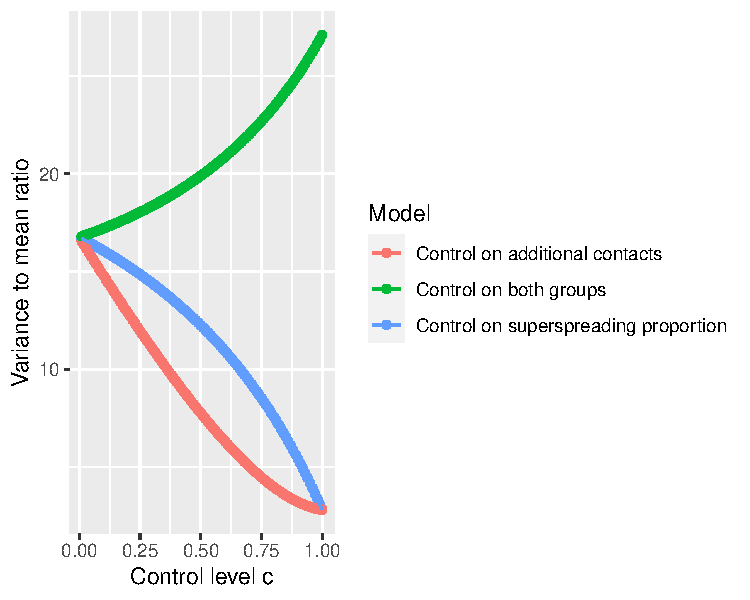
\includegraphics{Figure9.pdf}
    \caption{Control applied to both groups increases the variance-to-mean ratio in the number of secondary infections but control specifically targeted towards superspreaders reduces the variance-to-mean ratio in the number of cases, with control focused on reducing the number of additional contacts leading to the fastest reduction in case variability. }
    \label{fig:varmeanratio}
\end{figure}



%\section{Results}
% Figure 3: Coefficient of variation of distribution of secondary infections
% Figure 4: Probability of major outbreak
%Figure 5: Probability of observing a transmission chain of size <= 10
%Figure 6: CV chain size
%Figure 7: Effect of control activities: Control vs. Variance to mean ratio of distribution of secondary infections and  control vs. probability of extinction

\section{Discussion}

Our work shows that contact structure coupled with infectious period heterogeneity leads to overdispersed mixture offspring distribution. Our mechanistic model allows for infectious period distributions with a central tendency, which can retain the features of superspreading provided the influence of superspreaders in the overall population is strong, i.e., there is a large average number of additional contacts made per superspreader. We describe a flexible method for calculating the chain size distribution, which could be applied to other branching process models of infectious disease transmission. Our findings also suggest how individual-level behavior modifications and population-level control measures can affect critical thresholds for control.

Statistics generated using the mixture model \eqref{eqn:nbinommixpmf} differ substantially from those generated using the standard model if the population consists of a low proportion of superspreaders (Figures 5-8).  If the superspreading cohort has a large average number of contacts, the variance of the offspring mixture distribution and the probability of observing a chain size of one drives the difference between mixture distribution and the standard negative binomial model. Different offspring distributions induce different predictions for the frequency of large infection clusters. In their study of Poisson mixtures, \citet{Kremer2021-bi} similarly found that offspring distribution tail behavior depended on the model studied. We agree with their recommendation to compare different offspring distributions when fitting these models to data. 



Assuming that underlying dynamics can be described by a mixture model, the critical threshold for disease elimination depends on control strategy. The control strategies we explore target superspreaders by reducing the proportion of superspreaders (strategy (a)) or the number of additional contacts made per superspreader (strategy (b)) whereas strategy (c) is applied to the entire population. Our work suggests that directing control actions on all groups, e.g., via lockdowns, may be more suitable if the population is more homogeneous. We also show that elimination is only possible under strategies (a) and (b) provided $R_0$ of the pathogen in the regular cohort drops below one. This finding suggests that additional targeting of the cohort via population-wide measures such as stay-at-home orders may also be needed for elimination to be achieved. 


Our modeling approach has some limitations. We assume the same dispersion parameter $k$ for both groups in the population. For example, the superspreading cohort may have greater variability in the duration of their infections than the regular cohort. To allow for this, The model could be adapted so that the distribution of infectious periods in the superspreading cohort would be described by a lower dispersion parameter than that of the regular cohort. Our approach also assumes that the proportion of individuals that belong to each risk group can be identified \textit{a priori}. We expect that this would be achievable in closed settings such as care homes or in professional sports teams. Our approach yields a method for calculating the chain size distribution that may yield an analytical formula for some mixtures but for more complicated models such as the mixture model in this paper, it does not yield an analytical expression, which makes the approach less useful for model fitting to data.  


In conclusion, our model suggests that the addition of risk structure together with infectious period heterogeneity leads to variable outbreak dynamics, even if the infectious period has a central tendency. We recommend researchers examine mechanistic alternatives to the standard negative binomial model when studying outbreak distributions. 


 






\newpage

\bibliographystyle{amnat}
\bibliography{paperpile}
\end{document}
